\section{Segurança em Ambientes Hostis}
\begin{frame}{Segurança Cibernética em Ambientes Hostis}
    Tendo em vista o funcionamento de uma RSSF, outro aspecto essencial para seu funcionamento é a segurança. Os sensores, ao contrário de outros dispositivos de rede, correm riscos tanto digitais quanto físicos por conta de sua natureza e ambiente.

    \begin{exampleblock}{Exemplo: interferência eletromagnética}
        A exposição de sensores em ambientes veiculares pode causar interferências por conta do motor e outros equipamentos internos que geram ruídos eletromagnéticos, causando queda de desempenho na sensibilidade de transmissão e recepção de dados. O mesmo também cita que sinais de \textit{bluetooth} e Wi-Fi (WLAN) também podem degradar o desempenho dos sensores.
    \end{exampleblock}
\end{frame}

\begin{frame}{Ataques de Identidade}
    Numa RSSF, é praticamente impossível que todos os nós que não se conhecem tenham identidades convincentes. O ataque Sybill, conforme detalhado por Costa, Galetti e Pessanha (2024), consiste em atacar diretamente este ponto fraco da rede, onde um único \textit{hardware} assume múltiplas identidades em uma rede.

    
    Com isso, quando se usa um protocolo LEACH, o atacante consegue manipular sua chance estatística de ser eleito como líder (\textit{cluster-head}) por conta de suas várias identidades. Assim, ele pode criar um monopólio de segurança onde todos os dados de nós confiáveis passem primeiro pelo atacante, interceptando as transmissões.

\end{frame}

\begin{frame}{Ataques de Identidade}
    \begin{figure}
        \centering
        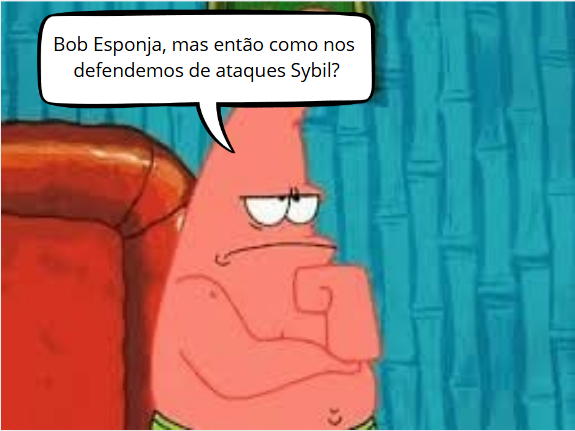
\includegraphics[width=0.58\linewidth]{figuras/patrick pergunta.PNG} 
        \label{fig:patrick pergunta}
    \end{figure}
\end{frame}

\begin{frame}{Ataques de Identidade}
    \begin{figure}
        \centering
        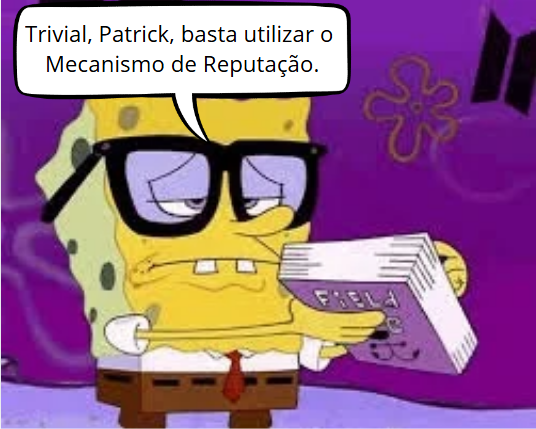
\includegraphics[width=0.55\linewidth]{figuras/bob esponja responde.PNG} 
        \label{fig:bob esponja responde}
    \end{figure}
\end{frame}

\begin{frame}{Estratégias de Resiliência}
    Tendo em vista como funcionam esses ataques, é necessário alguns métodos reforçados de segurança. Provavelmente a mais óbvia de se pensar seria o sistema de senhas e criptografia da rede, mas isso pode não ser viável por conta do alto consumo de energia e memória.

\end{frame}

\begin{frame}{Mecanismo de Reputação}
    Alternativamente, podemos usar o Mecanismo de Reputação, onde os nós observam o comportamento de seus vizinhos (como se estão enviando ou alterando pacotes de dados de forma suspeita). Nessa abordagem, cada nó mantém uma pontuação de confiabilidade dos seus vizinhos. Assim, se a reputação de algum vizinho cai abaixo de um limite, ele é simplesmente ignorado pela rede nas rotas de comunicação.

\end{frame}

\begin{frame}{Proteção da Camada Física}
    Entretanto, não é apenas a camada de rede que deve ser protegida, visto que o sinal dos sensores também pode ser alvo de ataque. Para resolver esse problema, a camada física foca em proteger a interceptação ou bloqueio do sinal de rede, adotando a técnica de espalhamento de espectro (FHSS/DSSS), na qual a ideia se baseia em ficar trocando a frequência do sinal. Dessa forma, caso uma frequência seja bloqueada, o sensor consegue trocar para outra.

\end{frame}